\documentclass[11pt,a4paper,footexclude,headsepline,footsepline,BCOR12mm,DIV13]{scrbook}
\usepackage[utf8]{inputenc}
\usepackage[english,german]{babel}
\usepackage{amsmath}
\usepackage{amsfonts}
\usepackage{amssymb}
\usepackage{graphicx}
\usepackage{styles/tumlogo}
\graphicspath{{images/}}
\usepackage{algorithm,algorithmic}
\usepackage{url}
\usepackage{hyperref}
\usepackage{todo}

\usepackage{bm} % Use \bm{\theta} 

\usepackage{mathtools}	% for small minus
\newcommand*{\matminus}{%
  \leavevmode
  \hphantom{0}%
  \llap{%
    \settowidth{\dimen0 }{$0$}%
    \resizebox{1.1\dimen0 }{\height}{$-$}%
  }%
}

\newcommand*{\matplus}{	% for small plus
	\text{+}
}

% remove indent after newline
\setlength\parindent{0pt}

% for rotated matrix
\usepackage{mathtools}
\usepackage{rotating}

% for pdf_tex
\usepackage{import}
\usepackage{xcolor}

\author{Anna Baumeister}
\title{Path Planning for an Ophthalmic Surgical Robot using V-REP}
\begin{document}

\thispagestyle{empty}

\vspace{4cm}
\begin{center}
  \oTUM{4cm}

  \vspace{5mm}
  \huge FAKULT{\"A}T F{\"U}R INFORMATIK\\
  \vspace{0.5cm}
  \large DER TECHNISCHEN UNIVERSIT{\"A}T M{\"U}NCHEN\\
  \vspace{1mm}

\end{center}


\vspace{15mm}
\begin{center}

  {\Large Bachelor's Thesis in Engineering Science}

  \vspace{20mm}

  {\huge\textbf{The Needle Detection and Reconstruction Based on OCT image with GPU Acceleration}}\\%[3ex]


  \vspace{15mm}


  {\LARGE  Anh Tuan Pham}


  \vspace{5mm}
  


  \begin{figure}[h!]
    \centering
    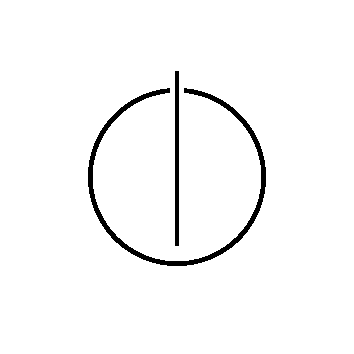
\includegraphics[width=4cm]{styles/informat.png}
  \end{figure}


\end{center}
\cleardoublepage
% The titlepage for the CAMP report document.
% Included by MAIN.TEX


% --------------------------------------------------
% The title page
% --------------------------------------------------

% correct BCOR - undo at the end !!!
% \def\bcorcor{0.15cm}
% \addtolength{\hoffset}{\bcorcor}

\thispagestyle{empty}

\vspace{7mm}
\begin{center}
  \oTUM{4cm}

  \vspace{5mm}
  \huge FAKULT{\"A}T F{\"U}R INFORMATIK\\
  \vspace{0.5cm}
  \large DER TECHNISCHEN UNIVERSIT{\"A}T M{\"U}NCHEN
\end{center}
\vspace{7mm}
\begin{center}

  {\Large Bachelor's Thesis in Engineering Science}

  \vspace{7mm}

  {\LARGE \textbf{Path Planning for an Ophthalmic Surgical Robot using V-REP}}\\

  \vspace{5mm}

  {\LARGE  	\textbf{Pfadplanung für einen Assistenzroboter in der Augenchirurgie mit V-REP}}\\

  \vspace{10mm}

  % \hfill
  \begin{tabular}{ll}
    \Large Author:     & \Large Anna Baumeister \\[2mm]
    \Large Supervisor:    & \Large Prof. Dr.-Ing. habil. Alois Knoll\\[2mm]
    \Large Advisor:	& \Large Mingchuan Zhou, M.Sc.\\[2mm]
    \Large Date:       & \Large \today
  \end{tabular}

  \vspace{5mm}

   \begin{figure}[h!]
     \centering
     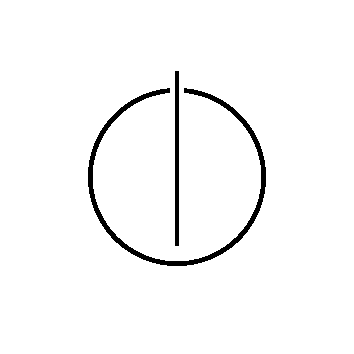
\includegraphics[width=4cm]{styles/informat.png}
   \end{figure}

  \vspace{10mm}

\end{center}

% undo BCOR correction
% \addtolength{\hoffset}{\bcorcor}

\cleardoublepage


%\thispagestyle{empty}

\vspace*{0.7\textheight}
\selectlanguage{english}
\noindent I assure the single handed composition of this bachelors's thesis only supported by declared resources.
\selectlanguage{german}

\vspace{7mm}

\noindent Ich versichere, dass ich diese Bachelorarbeit selbst\"andig verfasst und nur die angegebenen Quellen und Hilfsmittel verwendet habe.
\selectlanguage{english}

\vspace{12mm}

\selectlanguage{english}
\noindent Munich, September 14, 2017

\vspace{7mm}

\selectlanguage{german}
\noindent M\"unchen, den 14. September 2017 \hspace{3cm}  Anna Baumeister
\newpage
\selectlanguage{english}
\vspace{1cm}
I would like to thank my advisors Mingchuan Zhou and Professor Alois Knoll for their impossible patience and  aspiration. And to Mai Linh for proofreading this thesis with my horrible grammar. And to my mother, for supporting everything i do.

\cleardoublepage

\vspace*{2cm}
\begin{center}
{\Large \textbf{Abstract}}
\end{center}
\vspace{1cm}
In the recent years the medical world has witnessed a growing popularity of robot aided surgeries in various operations. This technical development has shown very promising results: Robot-aided operations are being done with better precision, miniaturization, decreased blood loss, less pain, and quicker healing time (?). 

Up to pace with the development, a robot with focus on eye surgeries is being developed by the Department of Robotics, TU Munich. The robot is designed to provide assistance in drug injections into the eye vessels, which is currently carried out by human surgeons. The complex nature of the human anatomy makes a needle penetration a challenging procedure. It requires a very high level of precision, whereas a small mistake could cause very costly damages to the eyes. Humans are not immune to errors, a tremor in the hands or a slightly suboptimal needle pose could not be totally prevented, and therefore a robot is particularly advantageous in this scenario.

One important part of robot development is to calculate the position and rotation of the needle at real-time, as accurately as possible. This task could demand a lot of effort. Ramona Schneider had successfully developed a robust algorithm in her master thesis to execute the calculation. The key element of this approach is to use Optical Coherence Tomography (OCT) images to compute the direction, x- and y-rotation of the needle. The remaining parameters, z-rotation and shift, are computed by defining intervals and combining values inside them. The combination with the most corresponding points is used for the transformation of the CAD model.

While the thesis showed great results, the execution still requires a lot of CPU resources and requires too much time for a real time system. Depending on the CPU used, the execution could take from 2 up to 3 seconds for each frame. The goal of this thesis is to find another approach to optimize the execution of the same algorithm, to reach a fastest execution time as possible.

Based on the nature of this algorithm, which is executing a lot of matrix calculations, a Graphic Processing Unit with far more superior number of threads available is more suitable for the task. In this thesis all of the calculations are executed parallelly on a GPU device with the help of OpenCL. Therefore the code was re-implemented in adjustment and optimization for GPU programming practice. The result is quite encouraging: for the same input and number of combinations, the optimized approach showed a 10x faster execution time, which is 20-30 milliseconds a frame without the best equipments. 


\tableofcontents{}

\chapter{Introduction}

\section{Objectives of this Thesis}
Subject of this thesis is the ophthalmic surgical robot developed in the iRAM!S project \cite{iramis}. When performing minimally invasive surgery, an important task is to prevent lateral movement of the tool at the point of incision to minimize strain on the surrounding tissue. In the iRAM!S project, this is achieved by defining a point on the needle as a Remote Center of Motion (RCM) and algorithmically forcing its velocity to zero. This thesis focuses on the following topics regarding the implementation of a virtual RCM:
\begin{itemize}
	\item Recalculation and verification of the Jacobian matrix for the surgical robot, both for unconstrained and constrained movement. For this purpose a model of the robot is implemented in the V-REP simulation environment.
	\item In the simulation environment, performing an injection at multiple sites of the inner eye surface and measuring the deviation of the RCM point  from its optimal position.
	\item Finding a set of control parameters that ensures that the needle pose quickly converges to any target pose within the workspace of the robot while maintaining the RCM position. 
	\item Comparing the performance of the Jacobian pseudoinverse method to V-REPs built-in inverse kinematics solver, which employs a Dampened Least Squares method, to get an estimate for the possible accuracy.
\end{itemize} 

\section{Robotic Assisted Minimally Invasive Surgery}

In recent years, robotic assistance has gained increasing acceptance in clinical practice, mainly due to improvements in precision, reliability and ergonomics. Most of these systems, referred to as \textit{surgical assistants}, are designed to enhance the ability of a surgeon to perform a certain procedure with additional tools. \textit{Surgeon extenders} are operated directly by the surgeon and offer improved instrument control and manoeuvrability by reducing hand tremor or offering more dexterous tool handling inside the patients body. The goal of these devices is to provide treatments for diseases that would be otherwise difficult to handle, decrease error rates and reduce the length of clinical procedures. Besides surgeon extenders, there are auxiliary surgical supports which operate along the surgeon and perform additional tasks such as controlling an endoscope. The surgeon can either steer the tool through an interface or the surcigal support may be autonomous to some degree. One of the most well-known robotic assistance devices currently used in clinical practice is the Da Vinci Surgical System \cite{DaVinci}.

\begin{figure}[t!]
	\centering
	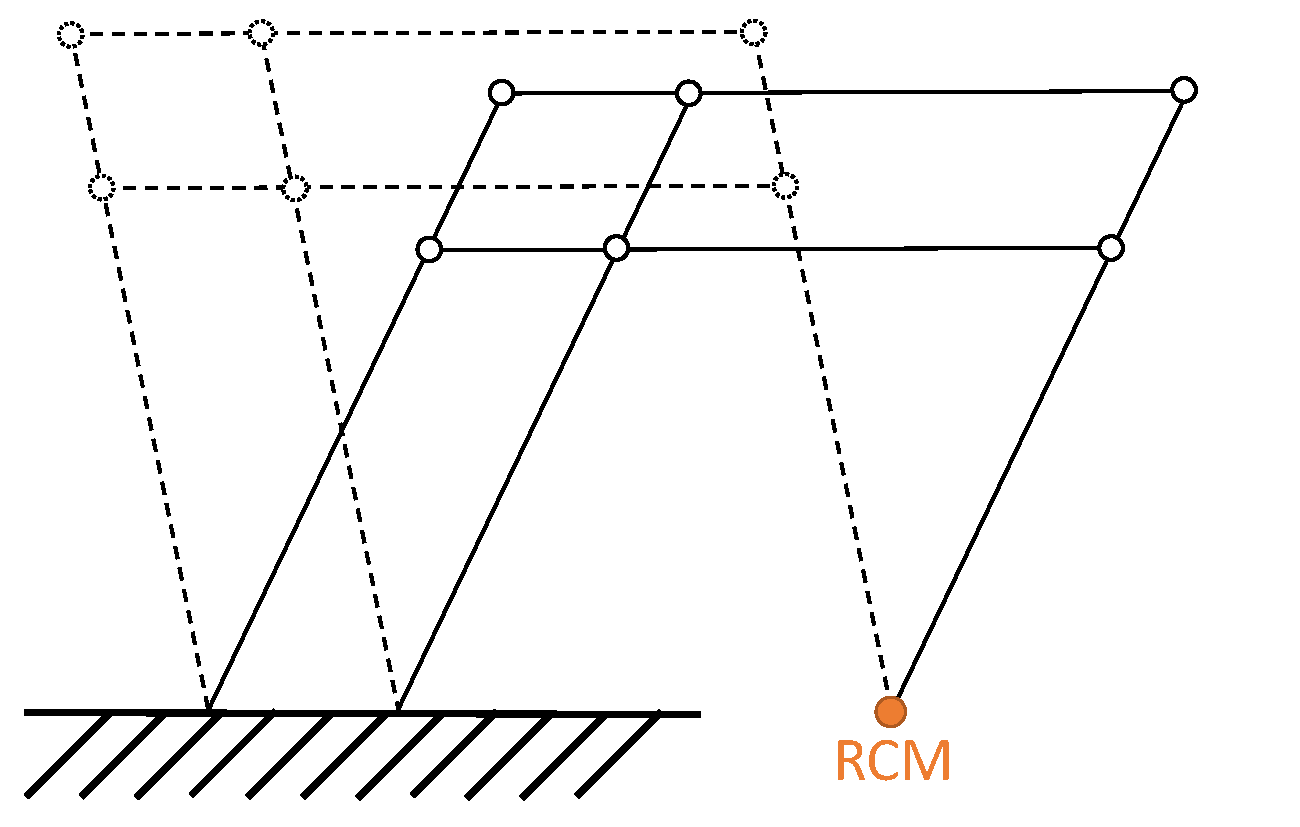
\includegraphics[width=6cm]{mechRCM}
	\caption{A simple, parallelogram based RCM mechanism. The RCM point is mechanically constrained and cannot move relative to the base frame of the robot.}
	\label{mechRCM}
\end{figure}
\begin{figure}[b!]
	\centering
	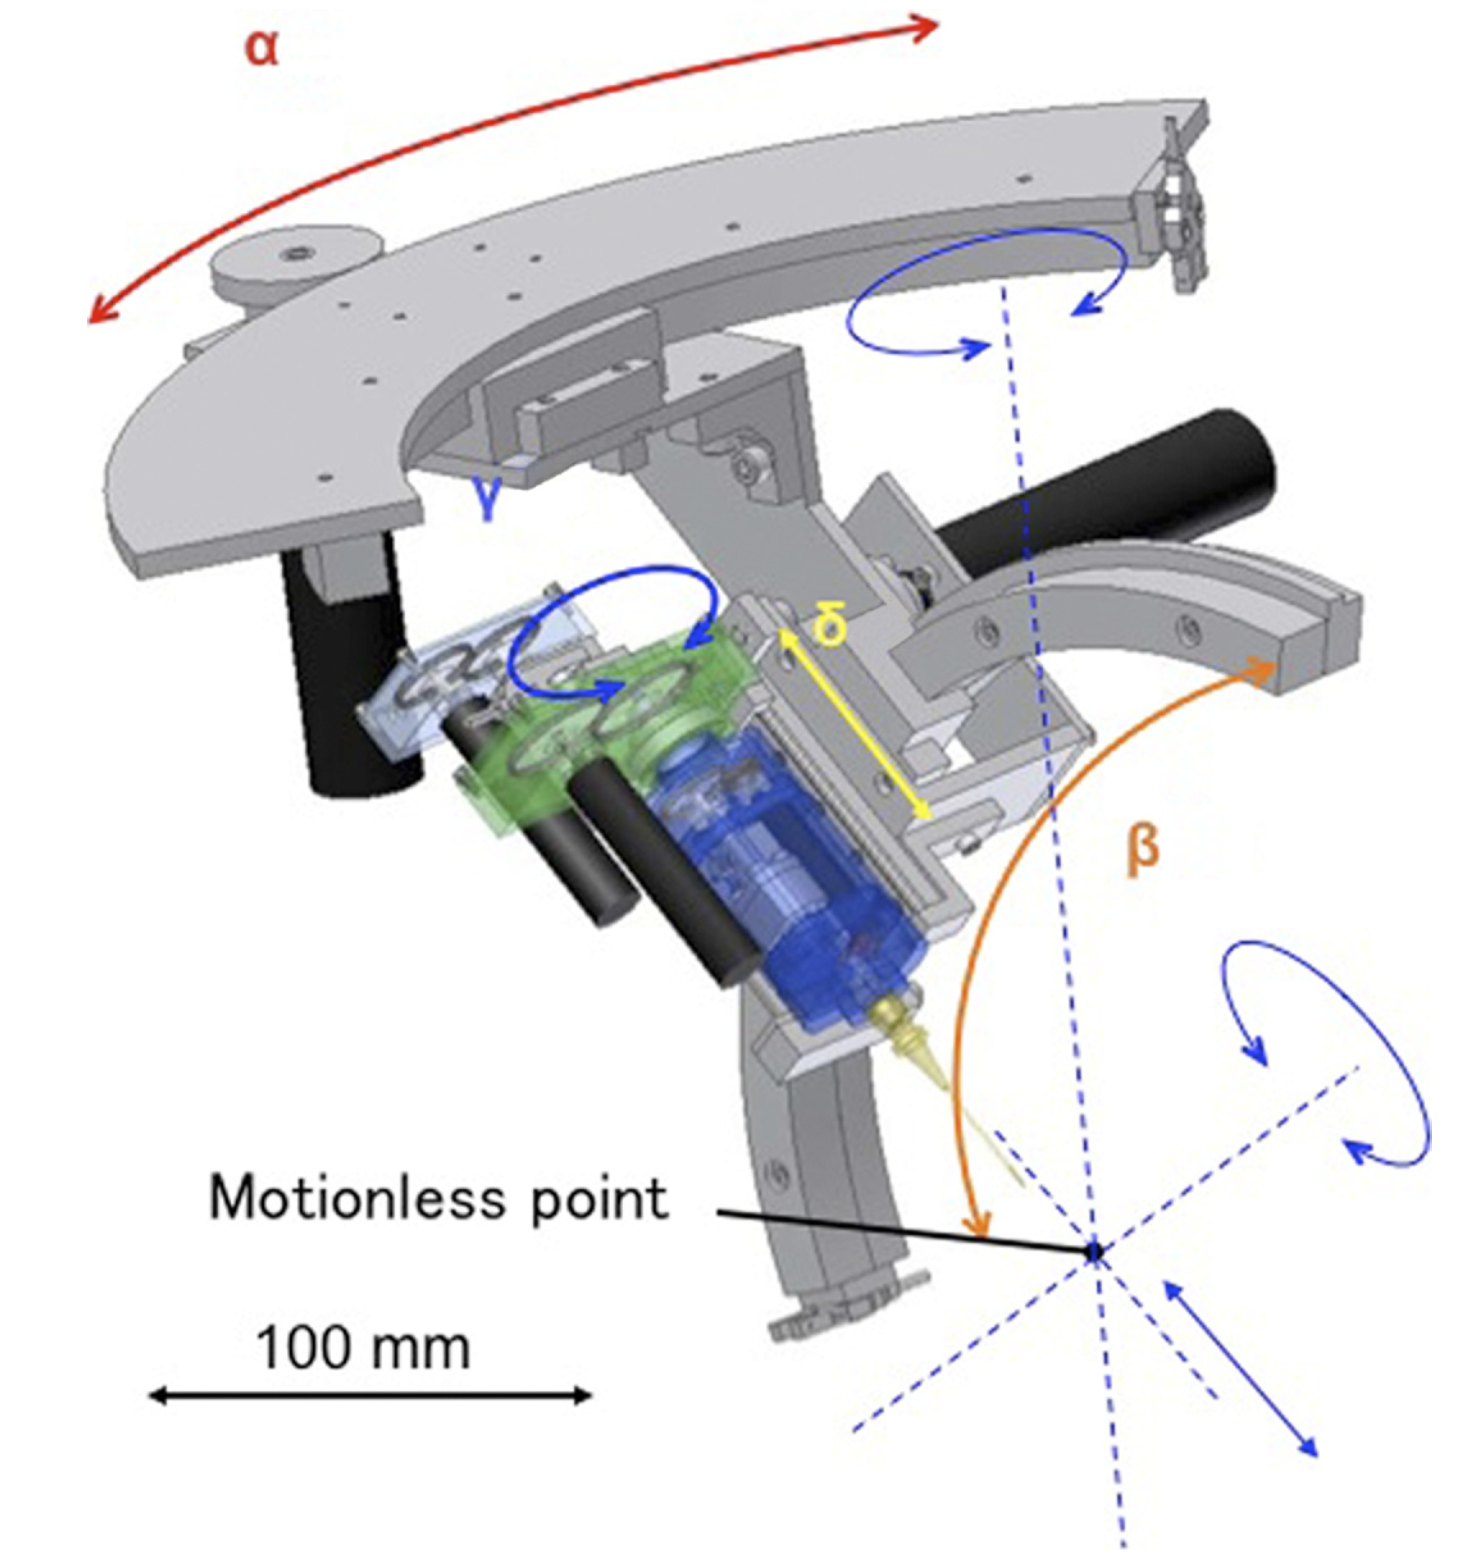
\includegraphics[width=7cm]{Ueta2017_robot}
	\caption{A mechanically constrained robot for ophthalmic surgery developed at the University of Tokyo \cite{Ueta2017}.}
	\label{Ueta2017img}
\end{figure}

Introduction of robots to clinical practice brings several benefits. One major point of interest is to provide smooth, tremor-free position control and force scaling for the tool. Robotic assistance seems especially promising in ophthalmic surgery, which relies on high precision to prevent damage to the delicate tissue of the eye. To minimize damage on the surrounding tissue, movement of the tool laterally to the point of incision must be prevented. While this is a challenging task for a surgeon it is comparably easy for a robot. This concept is referred to as Remote Center of Motion (RCM) and generally divided into two subcategories: \textbf{mechanically constrained} and \textbf{programmable} RCM. 

Examples for a mechanically constrained RCMs are shown in Figures \ref{mechRCM} and \ref{Ueta2017img}. Here, the RCM point is always in the same position relative to the base frame. Mechanically constraining the RCM point is superior in precision and reliability but offers little flexibility in ophthalmic surgery since the position of the robot defines the motionless point and consequently the patient or the whole robot need to be moved until the RCM point coincides with the point of incision.

A programmable RCM, sometimes referred to as a \textit{virtual fixture} \cite{MingLi2004}, is achieved by algorithmically forcing the velocity of an arbitrary point on the manipulator to be zero. This significantly increases the flexibility of the system, but also increases the complexity of the controller required to maintain high precision. Furthermore, a programmable RCM point is in general considered to be less safe than mechanically constrained systems.

The iRAM!S project \cite{nasseri2013introduction} is a joint collaboration of the informatics institute \textit{Robotics and Embedded Systems}, the Graduate School of Information Science in Health (GSISH) and the TUM university hospital Klinikum rechts der Isar. The goal of the project is the development of a novel robotic system for assisting ophthalmic surgeons in complex retinal surgeries, for example for the treatment of diseases such as retinal vein occlusion.

\begin{figure}[t!]
	\centering
	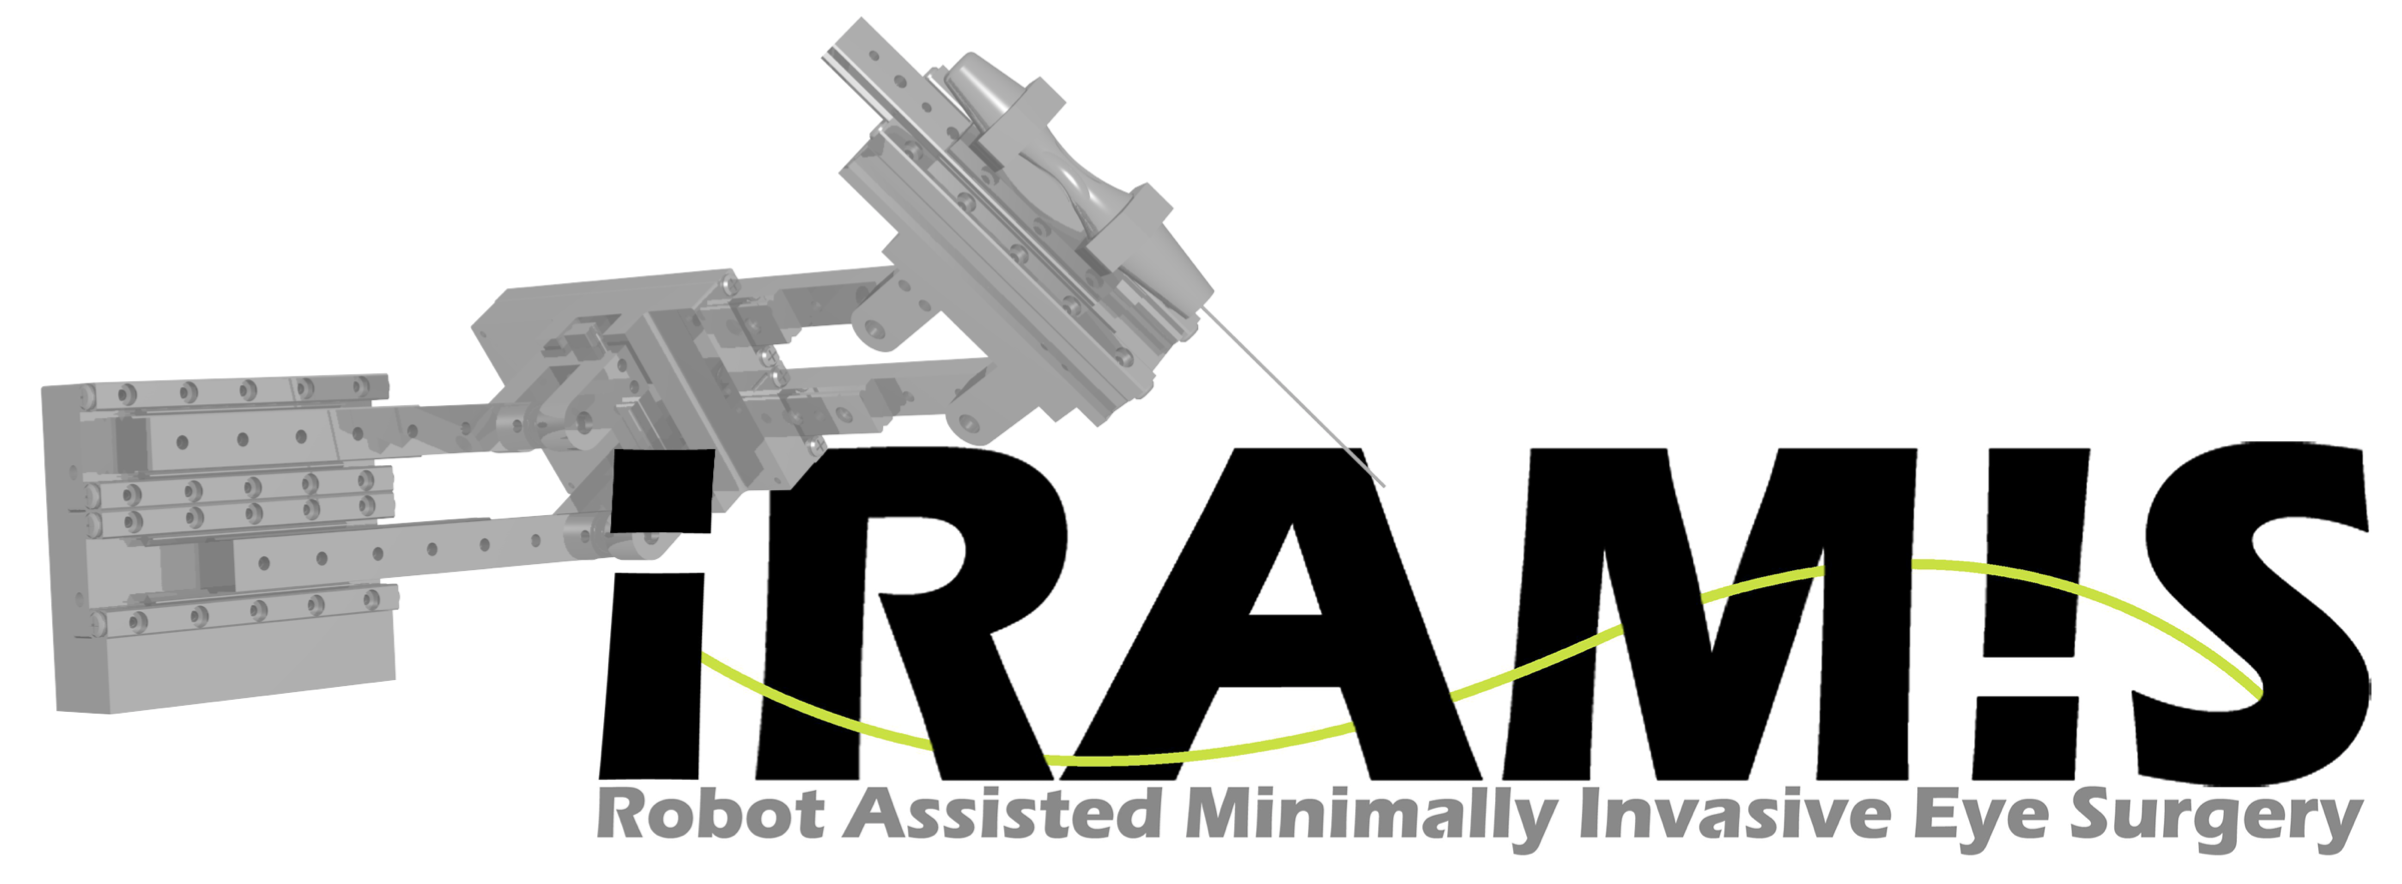
\includegraphics[width=12cm]{iRAM!S}
	\caption{The robotic assistant for ophthalmic surgery developed within the iRAMI!S project \cite{iramis}.}
	\label{iRAM!S}
\end{figure}

\section{Outline}
The second chapter of this thesis describes the mechanical design of the robot and reviews the kinematic relations between joint movements and end effector pose. A step by step description is presented on how to derive the Jacobian from the Denavit-Hartenberg parameters of the robot. 

The Jacobian pseudoinverse approach as a solution for the inverse kinematics problem is introduced, along with the concept of the \textit{augmented Jacobian matrix}, which is used to implement the Remote Center of Motion constraint. Finally, there is a brief introduction to the simulation environment V-REP which will be used to validate the results of the thesis.

In the third chapter, the extended robot task and corresponding Jacobian matrix is defined. A V-REP simulation model is designed from the CAD file and controlled both via a MATLAB remote API and a child script using V-REPs built-in inverse kinematics function. 

In the final Section, the precisions and execution times of both methods are evaluated and compared.
\chapter{Open Computing Language}
The focus of this thesis is to adapt the well reviewed, functional algorithm into the context of GPU programming practice with the help of Open Computing Language (OpenCL). Normal software often runs on processors, which could provide a very high clock speed but a rather small number of threads, hence a graphic card could perform much better at certain tasks. The design of a graphic card allows it to be very efficient at graphic manipulation, image processing etc.. In the following section of the thesis the design and specification of a graphic card is introduced to provide an insightful overview of how it works and why it is important to have the right configuration for the best possible performance.  
\section{Graphic Processing Unit}
Graphic processing units (GPUs), which is defined as "a specialized electronic circuit designed to rapidly manipulate and alter memory to accelerate the creation of images in a frame buffer intended for output to a display device"\cite{wikipedia}, are widely used in modern devices such as computers, embedded systems and gaming consoles. GPUs have a highly parallel architecture and a very high number of cores, which make them very efficient on tasks that can be highly parallelized, such as matrix calculation, image processing etc..  For example, the latest Intel central processing unit (CPU) Core i9 has only 6 cores and 12 threads while the latest GPU by NVIDIA, the GTX 1080, has 2560 Cores, which is around 400 times the number of cores of the i9.

Although each core of a CPU could show a superior clock speed, which is 2-3x faster than a GPU core depending on type and generation, a GPU has far more cores to work with. For tasks that could be divided into smaller subtasks and executed in a parallel way, using GPU often shows a much better result.

In our thesis, the transformation of points with transformation matrices is a task that is very independent and repeating. Therefore running a shifting algorithm with the help of a CPU is very disadvantageous, mainly due to two reasons:

\begin{itemize}
	\item CPUs in single CPU systems are normally preoccupied by another process in an operating system. Depending on the cores and threads available it is not possible to fully parallelize all combinations even with server oriented processors. Therefore the combinations, which could be several hundreds, would be executed one after each other.

	\item GPUs, on the other hand, can be used as a dedicated unit for the task only. It is even possible to use more than one GPU at a time, in case the number of threads needed are higher than those that are available. The high number of work units allows the calculation of each combination to be further divided into smaller task and parallelized.
\end{itemize} 

With those advantages, an implementation with the GPU, when done right, could be much faster than running the tasks with a CPU. Furthermore, combining the two type of units is a great solution for the task at hand, since OCT image processing still needs to be done with CPU. 

One important difference in GPU programming is memory management. Unlike CPU, the GPU can not access memory directly from RAM, but it has its own memory, which could vary from 1GB to 8GB. There are three types of memory relevant for GPU programming: global, local and private memory. These three types have very different access speeds with private memory being the fastest and global memory being the slowest type. Furthermore, an extra step is needed to transfer memory such as arrays to the memory of the device. To improve the efficiency of the program, it is not only critical to allocate and use the memory wisely, but also to minimize the amount of memory transferred as well as the total count of transfers. The difference a well managed memory usage makes could be unnoticeable with a smaller amount of memory, but could be significant when using a larger amount of memory, for example an array of millions of floats. In the next sections a closer explanation of these memory types will be taken to understand the importance of using them right.
\pagebreak
\section{OpenCL Framework}
OpenCL is a framework for writing programs that can be executed across heterogeneous platforms. It can run with CPUs, GPUs, digital signal processors, or other hardware processors on computers, servers or mobile devices. OpenCL provides an interface to control platforms and devices and execute programs on those available devices. It often provides great boosts in performance based on parallel computing with task and data-based parallelism. The following listing shows the structure relation between host, compute devices and processing elements within \cite{opencl}. By this model the terminologies will be explained further in the later sections.
 

\begin{figure}[H]
	\centering
	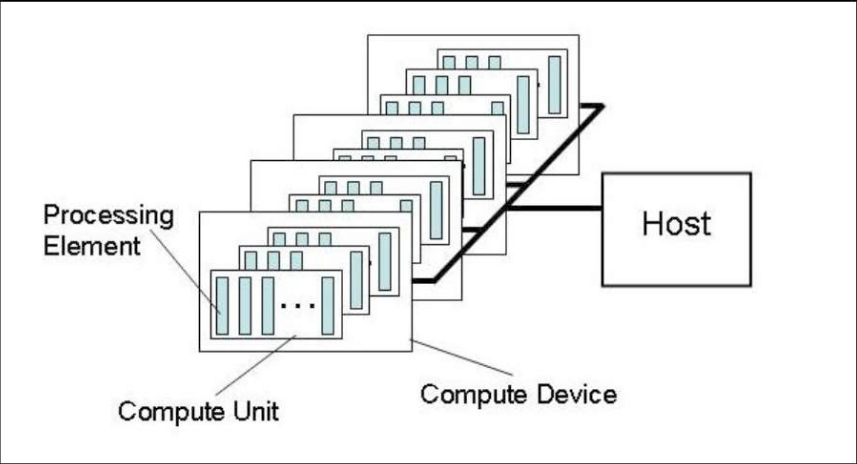
\includegraphics[width=8cm]{images/OpenCLModel.png}
	\caption{An examplary OCT image of the needle}
	\label{ExampleOCTImage}
\end{figure}
\pagebreak
\subsection{Platform}
A core concept of programming with OpenCL is platform. A platform consists of a host and one or more connected devices, in this case OpenCL supports GPUs. A connected device is then further divided into compute units and processing elements. How many processing elements  are grouped into one compute unit varies between vendors and is a relevant factor for the optimization of the OpenCL program. 

An OpenCL application consists of two types of code: host code and device code. The host code is run by a host processor with the objectives of creating a platform, prepare data, transfer data to the device and ultimately send commands to the devices. The device code, also known as kernel code, is the piece of code that will be read and executed by the device only. There is a restriction of device code: it can only be written using C standards, meaning external libraries or methods will not be accepted in kernel code. 

Unlike CUDA, an equivalent implementation of NVIDIA, OpenCL can be used for any device that supports the API. CUDA reportedly has a slightly better performance because it was  designed exclusively for NVIDIA GPU, hence optimized with the architecture, but OpenCL offers more flexibility with a competitive performance. 
\subsection{Memory model}
The OpenCL memory model is composed of three layers, global memory, local memory, work group memory. The difference between those memory types is how accessible they are to a single processing unit. Global memory can be accessed by any processing unit, but is also the slowest of the three. Local memories can be accessed from processing units that are in the same work group. Every processing unit has a certain amount of private memory, which can be accessed by that unit only. From top to bottom of the memory hierarchy, the size of memory available for global, local and private memory reduces hierarchically. A more concrete presentation of the relationship between processing units could be roughly presented as follow, only roughly accurate because of different specifications between AMD and NVIDIA \cite{openclplatform}:

\begin{figure}[H]
	\centering
	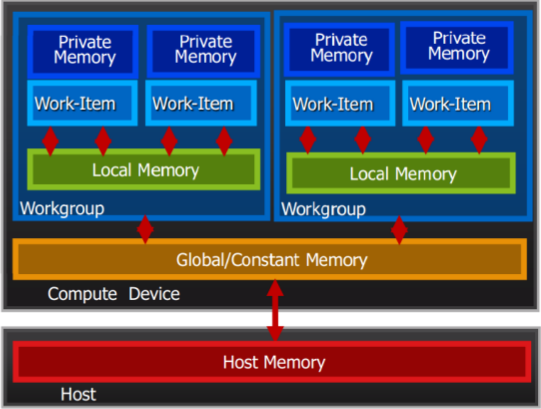
\includegraphics[width=8cm]{images/Model.png}
	\caption{Memory Hierachy}
	\label{ExampleOCTImage}
\end{figure}

\subsection{Execution steps of a OpenCL Program}
OpenCL API allows program to be platform independent, that means it would work with every devices that supports the API. Users can actively manage task, choose device they want to execute the task on and commence execution without deep knowledge of the hardware layer. It does however requires some preparation steps from the host to configure the OpenCL Model. The steps should be carried out in order as following:
\begin{itemize}
	\item Accessing Platform: The step of choosing which platform to execute the kernel code on. OpenCL provides a data structure named cl\_platform\_id and a method clGetPlatformIDs to assist with the issue. Calling clGetPlatformIds with a result array as arguments results into an array of available platform. Users can also define how many platforms they are looking for and the function uses it as a boundary for the search. Furthermore, more detailed information about a certain platform will be presented with the help of function clGetPlatformInfo (Vendors, Version, Profile et cetera).
	\item Accessing Device: Once the Platform has been selected, users can access all the available devices in the machine. A device is represented with cl\_device\_id data structure. Similar to the previous step, a method is provided to enlist all the devices available: clGetDeviceIds. Optimization often requires specification such as work size and the work group number of the device being used. This is where clGetDeviceInfo becomes very useful: it provides all the specification of the selected device.
	\item Creating Context: To add command queue and execute it, a context must be created for the selected platform. The context from a platform can only accept devices from the same platform’s vendor. It means an AMD GPU and an NVIDIA GPU can not run on the same context, there must be two for each of them. Context is represented by cl\_context data structure, which could be created using clCreateContext() or clCreateContextFromType().
	\item Creating Program:  After gathering all the information needed about the hardware, it is time to create the OpenCL Program. A Program is a cl\_program data structures which holds all the kernels together. In order to successfully create a program, a source file or a binary file storing all kernel method is required. Then depending on which kind of source file is being used, clCreateProgramWithSource() or clCreateProgramWithBinary() should be used to create the program. 
	\item Build Program: The created program still needs to be built, or differently speaking to be compiled by OpenCL Compiler, which must be done with clBuildProgram() method. This step could be very troublesome as the compiler expects the source file to contain kernels without syntax errors. In case there is one the build will fail and return -1. To ease up the kernel debugging process there is an option of using clGetProgramBuildInfo() to print out a trace of all possible problems the compiler could find in the kernel code.
	\item Creating Function kernels: Unlike traditional programming practice, methods can not be called directly, but need to be packed in a cl\_kernel data structure first. Every function that will be called needs to be packed in a kernel object and these objects can be reused multiple times. Alternatively an array of kernels could be created and packed by using clCreateKernelsInProgramm(). 
	\item Setting arguments for kernel:  In case there are function arguments, these must be added into newly created kernel objects. Every argument should be packed into a cl\_mem object, which can be created by using clCreateBuffer(). Using this method, programmers have the choice of how the memory should be created and initialized, if it should be read only or read and write, or write only. These options are made available by implemented flags inside the function. Performance differences between those options could be very high for a real time system. The main reason behind the difference is how the memory should be initialized, by default or by user input. In the case of user initialized memory, it takes time to transfer from host to device, which depends on the speed of the computer’s PCI Express. Memory transferring between host and pointer is generally a slow process in proportion to internal memory access speed, hence it is recommended to reduce the amount of memory transferred as much as possible. Another reason for caution in this step is to define the right amount of memory required, because if the size of the memory created is smaller than needed, the program will still function and give back unexpected behavior which could be hard to debug. After creating the cl\_mem buffer object, it is still necessary to tell kernel objects which buffer object belongs to which kernel function and the corresponding index of the arguments in function. OpenCL API provides the function clSetKernelArg() to bind the buffers to the arguments of kernel. The parameters needed for this function are the index of corresponding argument value, size of buffer object and a pointer to the buffer.
	\item Creating Command Queue: The execution of kernel methods must be managed by a command queue. Given the context and program created in previous steps, a new command queue could easily be created by using clCreateCommandQueue(). The method returns a cl\_command\_queue object and its reference count could be retained by clRetainCommandQueue() or decremented with clReleaseCommandQueue(). The queue follows the first-in-first-out principle, meaning a task that was added first into the queue will be executed firstly.
	\item Enqueue Kernel: The purpose of this step is to set the created arguments to the kernel object to an queue and execution.  There are two functions created to accomplish this task: clEnqueueTask() and clEnqueueNDRangeKernel(). The first one, clEnqueueTask, is not frequently used in real world OpenCL application. It only allows to execute kernel within one single work item, which is not the point of parallelism. In fact it was only used in tutorials as introduction to OpenCL. The second one, clEnqueueNDRangeKernel() is more complicated and widely used. Within this function, users can define the dimensions of work groups, local work size, work offset, et cetera. These factors will be explained further in the next chapter about what they are, and why they play an important role in overall performance. After calling this function, the command will be executed in the device. On a further note, if there are severals kernel on the queue and each one of them needs to be executed before moving on to the next, clFlush() and clFinish() should be called right after.
	\item Reading from Buffer Object: After executing kernel, users can read the result from the buffer objects, which could be done by calling clEnqueueReadBuffer(). In this method, the buffer object, a destination array (allocated memory for large arrays to avoid segmentation fault), a size of the memory to be read, and in some case, offset, should be defined. The function returns 0 when executed properly without error.
\end{itemize}

These steps are required to run an OpenCL Application properly. Every method mentioned allows the user to define a variable for storing and debugging error code. As usual, 0 means everything works, other numbers indicate an error. There are various types of error codes, which are also listed by OpenCL specification, of why and where they happen. However, these steps do not need to be repeated every time users want to run another kernel command. Step 1 - 5 are only needed to run once after the program starts as preparation. It should only be run once, because the time needed to compile kernel code from a source could be very slow. In this thesis, when a performance time is mentioned, it is also implied that the preparation steps are not included, because they only need to be executed after the start up. As discussed before, there are some parameters that need to be configured in these steps to improve the performance of the program, but before going into details about those configurations, a good understanding of work group and work items is required, which will be the focus of the next chapter. 

\subsection{Global, local work size, work groups}
The difference the GPU programming makes in comparison to the CPU is the ability of running many more threads at the same time. In the steps described in the previous chapter, there is not yet a defined number of threads to be executed. The first question to be answered before trying to parallelize a program is how many threads are needed. For OpenCL it does not matter how many threads the users want, the program will execute anyway because of its management mechanism. The reason behind this is that if the number is more than the ones that are available, OpenCL will execute those surplus threads as soon as there are threads available again. This, while being very flexible, eliminates the advantage of parallelism.

Secondly, knowing how many work items are available, assuming the device is not preoccupied by graphical task of the computer, is important for designing the program. As mentioned before, OpenCL provides the method clGetDeviceInfo() allowing users to have a closer look into the specification of the device. Furthermore, users can run the command “clinfo” to access the full information about all the platforms available from the terminal, given that OpenCL is installed correctly. The result will be a list of platforms and the devices available in each platform, the specification of these devices with critical information pieces like Vendor, Version, Version of Supported OpenCL, Clock frequency, et cetera. In this chapter, “Max work item dimensions”, “Max work item sizes”, “Max work group size” will be discussed further. The following picture shows an example of the result when clinfo is called:

\begin{figure}[H]
	\centering
	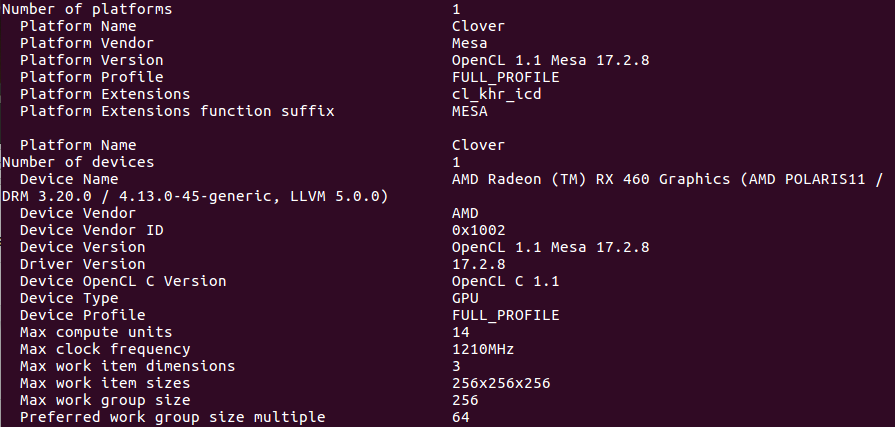
\includegraphics[width=12cm]{images/clinfo.png}
	\caption{Information about current available devices}
	\label{ExampleOCTImage}
\end{figure}

Threads in the GPU programming world can also be called as work items, since work items are meant to be executed parallelly. For the sake of simplicity the device shown in the last picture will be used as an example. In this example it is a low end AMD graphic card and has the max work item size of 256x256x256. The numbers show the max number of work items available in each dimension. It is similar to a 3D coordination system and hence the number of all work items available can be calculated as: 256 x 256 x 256 = 16,777,216 work items. In comparison with off the shelf CPUs, the number of work items of a GPU is far more superior.

In the scope of this thesis, the number of threads available is far more than what is needed (around 1-2 million work items). It is still necessary to inform OpenCL the number of threads the application needs, which leads to the definition of global work size. Global work size is basically  the number of threads a user needs. It does not have a limit, meaning a user can define the global work size as much as they like, as long as the device global memory is not exceeded. The global work size can have as much as three dimensions, but it does not necessary need to. For some special tasks it would be very practical to use more than one, for example image processing with two work size dimensions. But in all cases, using one dimension is intuitive, sufficient and often more advantageous for optimization, which will be explained later. Following is a simplified presentation of work group and work items\cite{openclplatform}

\begin{figure}[H]
	\centering
	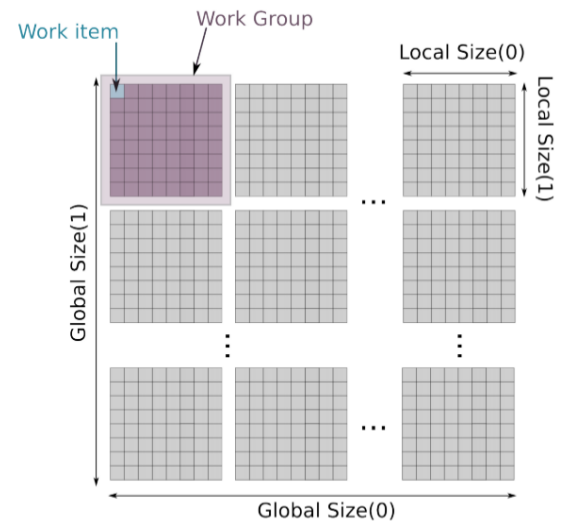
\includegraphics[width=10 cm]{images/itemunit.png}
	\caption{Information about current available devices}
	\label{ExampleOCTImage}
\end{figure}

On the other hand, local work size can not be as arbitrary big as users want, it is constraint by the specification of the device. The limit of the local work size is also defined by the max number of work items per dimension, in the example it is 256 items per work group per dimension. Unlike the global work size, it is not obligatory to define the local work size, users can define it as NULL if they wish to. In this case, OpenCL will handle the local work size itself.

A work group is basically a set of work items that are grouped together. The number of work group can be dynamic, as it depends on the number of the global work size and the local work size. Grouping work items together can have certain positive effects on the performance, since work items in the same work group are synchronized much better and can have access to local memory, which could be advantageous. It is also critical to set the global work size to be a natural multiple of the local work size. For example, if a local work size of 128 is defined, then the global work size must be 128*n where n is a natural number.

Each GPU vendor has developed their own optimization strategy with a prefered local work size definition. As mentioned before, the only constraint between the local and global work size is only that the local work size should be the natural divisor of global work size. Configuring the right local work size has a positive impact to the overall performance. NVIDIA recommends for their GPUs a multiple of 32 for local work size, while for AMD equivalent the recommendation is a multiple of 64. (SOURCE). The reason behind the performance improvement is the architecture of the GPU: A wavefront (fundamental work unit of AMD GPUS) consists of 64 work items, thusly a multiple of 64 local work size will not require a regroup of work-items, therefore provides better performance. The same explanation applies to NVIDIA GPUs.

Global, local work size and work group are very important terminologies in GPU Programming. A good knowledge and correct information of the specification of  the device can boost up the performance quite significantly.
\newpage

\subsection{Kernel}

As explained previously, kernel code is the piece of software that is actually executed in the device. Writing a comprehensive, efficient and error-free kernel code can be quite challenging for programmers without previous low level programming experience. The most important aspects of kernel code is the private memory management, syntax, and utilisation of available memory. One important aspect to be concerned about is that the resource (memory, calculating power) available for one work unit is very limited. This explains why it is very important to reduce the workload in each kernel function as much as possible.

There are several constraints to be concerned about while writing a kernel function. The following code snippet is an illustration for a simple kernel method with OpenCL. The function adds two elements of two arrays and write the result to a third array:
\begin{lstlisting}[language=C]
__kernel void hello(__global int *a, __global int *b
						, __global int *c) {
        int gid = get\_global\_id(0);
        C[gid] = a[gid]+b[gid];
}

\end{lstlisting}

Every kernel function, with an exception of auxiliary functions, must have the identifier “\_\_kernel” and void as return value. Passing parameters consists of three arrays, all of them have “\_\_global” as identifier, indicating the source of the arguments. There are three different kinds of identifiers in the memory model as mentioned before: “\_\_global”, “\_\_local”, “\_\_private”. Note that it is required to pass pointers to the function, regardless what data type it is: an array, an int, float or a customized data structure.

There are some built in options of array representation in OpenCL. For each primitive data type there are severals options to represent an array with that type with a predefined size, for example: float4, int4, char4 et cetera. Users can also use normal array structures used in the C programming language.  As previously discussed, the maximum size of arrays is quite limited due to the lack of memory available. It is recommended to use global or local memory depending on the required array length. Following listing shows an example of TODO

In kernel function, it is impossible to use functions from external libraries. However, the API supports standard C library with its useful arithmetic functions like max, min et cetera. With more complicated functions, for example the correspondence matching function which will be later implemented, it is recommended to divide the function into smaller parts and rewrite it into C conformed functions. It is often the case that a piece of code is quite often reused in kernel, therefore programmers have the possibility to pack it into an auxiliary function, which still follows the principle with identifiers for passing arguments.

The execution model of OpenCL works on the principle that every work item knows what to do and can be independent on the work of other work items. On the very first line of the code, the function get\_global\_id() is called and saved as an index for the elements to be added. The function call returns the unique work item index of the first dimension of work sizes (index starts at 0), since in this sample only one work dimension is used.

One big challenge of writing kernel in OpenCL is the lack of a built in debugger tool or the possibility of  looking to the steps that are being taken. However, there are several external programs that could be helpful for analyzing, profiling the application like CodeXL, GPUVerify from the Imperial College of London or Oclgrind from the University of Bristol. These applications allow users to run kernel with customized arguments, profile execution time, running kernel step by step. However, having a good strategy for parallelizing is the best way to prevent errors in execution.

\chapter{Shifting Algorithm with OpenCL}
This chapter focuses on the mentioned shifting algorithm, the hardware used, inputs, the result and optimization techniques. After understanding the fundamentals of OpenCL, it is important to choose a strategy to divide into smaller tasks and implement it in OpenCL. The shifting algorithm will be repeated in four iterations with adjustments after each iteration to reach the best results. 

\section{Hardware}
This chapter focuses on the mentioned shifting algorithm, the hardware used, inputs, the result and optimization techniques. After understanding the fundamentals of OpenCL, it is important to choose a strategy to divide into smaller tasks and implement it in OpenCL. The shifting algorithm will be repeated in four iterations with adjustments after each iteration to reach the best results. In this thesis, two sets of hardware are used for running the application:

\begin{lstlisting}
	Set 1    
    CPU : AMD Ryzen 5 1600X
    Graphic card : AMD RX 460
    PCI Express 3
    Memory : 16 GB

\end{lstlisting}

\begin{lstlisting}
	Set 2    
    CPU : Intel Core i7 7700K
    Graphic Card : NVIDIA TITAN X
    PCI Express 3
    Memory : 16 GB

\end{lstlisting}

The components in set 1 are not the best components in the market. A better combination of high end components (set 2) can improve the component significantly. 

\newpage
\section{Program Input}
Adopting results from the first part from Ramonas work, the shifting algorithm is responsible to find a shift-rotation combination with the highest number of matching points. As input there are the original point cloud, the CAD model point cloud and initial guess transformations and specifications of shift-rotation combinations. These specifications are: angle interval, shift interval, step length in two dimensions (shift and rotation). These information are deciding factors for the amount of possible combinations and therefore workload.

In the thesis a data set is used as a test set for the program. The two point clouds, a CAD model and a constructed model (from OCT Images), consisting of 2289 and 1225 points respectively. As discussed before, a point cloud data structure can not be used in the context of kernel code, so a conversion is needed to make data transfer possible: For each point cloud, an array of float is thrice the size of the mentioned point cloud is created to store the coordination of the points included. In this case the arrays are created with the sizes of 6867 (2289*3) and 3675 (1225*3). Because of the rather big sizes, the memories are allocated in dynamic memory to avoid segmentation fault error.

The initial values of the interval length, step length, and initial angles and shift, are adopted from the first part of the thesis. After each iteration these values are adjusted to the best result to move on to the next iteration. Initially the angle interval of 10.0 grad with a step length of 1.0f and a shift interval of 0.5f with step length 0.05f were chosen. From these specifications we have a number of angle steps, calculated as following:

\begin{equation*}
Num\_angle\_step = 10/1 +1 = 11;
\end{equation*}
And a number of shift steps:
\begin{equation*}
Num\_shift\_step = 0.5/0.05 +1 = 11;
\end{equation*}
With 11 angle steps and 11 shift steps, the total number of all combination is the production of the two, which results in 121 combinations. In the first round of four iterations, there are 121 of combinations to be transformed, calculated and served as candidates for the best result. These basic information are critical for the implementation, the reasons behind will be discussed later.
\newpage
\section{Process}

Given the point clouds and the initial translation, one iteration of Iterative Closest Point can be processed in roughly four steps, which will be repeated for each combination of shift-rotation:

\begin{itemize}
\item Computation of transformation matrix using the initial translation and rotation based on the shift and angle step of the combination.
\item Translate the model point cloud with the new transformation matrix. 
\item Calculating the number of matching points between the transformed point cloud and OCT generated point clouds. A matching point is found if the distance between that matched point and the source point is closer than a certain threshold. In the thesis the threshold was defined as 0.02f.
\item Analyzing the results to determine the combination with highest number of matching points. Using the newly found combination as pivot to calculate the next interval for shift and rotation and applying these intervals for the next iteration.
\end{itemize}

The results of the described process is an array of combination index - number of matching points.  The next step is to find the combination which holds the highest number of matching points and retrieve the corresponding angle step and shift step with the combination. The new found angle step and shift step will be used as pivot to compute the angle and shift interval for the next iteration. The step lengths are also reduced after each iteration to improve the approximation. Unconstant shift and angle intervals and changing step lengths account to unpredictable number of combinations in the next iterations. 

After four iterations the best combination is considered as the end result which converges to the actual position, a corresponding rotation and translation is computed and the process is therefore finished.

\section{Concrete implementation}
In GPU Programming, it is important to choose a strategy which part to parallelize. Understanding the difference and device specification, in this chapter we will take a closer look of how the previously described steps are executed.

In the OpenCL implementation, the steps are differently grouped but the fundamentals stay the same. The first and second step, which are responsible for calculating the transformation and transform the point cloud. The second step can not take place without the first being finished, hence the reason why these two steps are not parallelized. For an intuitive demonstration of the algorithm, the numbers used in the next chapter are based on the test data set.

\subsection{Transformation matrix calculation and apply to point cloud
}
Adopting the method used in Ramonas work, the transformation matrix can be calculated knowing the shift and the angle step. The 4x4  matrix consists of one 3x3 rotation matrix and a 3x1 translation vector, the last row is always defined with a (0,0,0,1) vector, regardless of the angle and shift step. 

The rotation matrix can be calculated as follow:

\begin{lstlisting}
rotating[0] = cos(angle_temp);
rotating[1] = -sin(angle_temp);
rotating[3] = sin(angle_temp);
rotating[4] = cos(angle_temp);
\end{lstlisting}

Whereas rotating is an array of float with size 9 (represents 3*3 matrix) and angle\_temp is the angle of current combination, which is:
\begin{lstlisting}
angle_temp = (angle_min+angle*angle_step)*(0.01745328888);
\end{lstlisting}
Then the first elements of transformation matrix can be calculated as follow :
\begin{lstlisting}[language=C]
transform[0]= floatArgs[12]*rotating[0]+floatArgs[13]*rotating[3];
transform[1]= floatArgs[12]*rotating[1]+floatArgs[13]*rotating[4];
transform[2]= floatArgs[14];

transform[4]= floatArgs[15]*rotating[0]+floatArgs[16]*rotating[3];
transform[5]= floatArgs[15]*rotating[1]+floatArgs[16]*rotating[4];
transform[6]= floatArgs[17];

transform[8]= floatArgs[18]*rotating[0]+floatArgs[19]*rotating[3];
transform[9]= floatArgs[18]*rotating[1]+floatArgs[19]*rotating[4];
transform[10]= floatArgs[20];
\end{lstlisting}

It is worth noting that the default values of a float array is 0.0f, it is the reason why all others indexes do not have value assignment. Furthermore, with the knowledge of constant array values, some arithmetic operations can be neglected without changing the end result, for example multiplication with 0.0f. Reducing these redundant assignment and operation has a significant impact on the performance, since the clock speed of each unit is not very high in comparison to CPU cores. 

Applying the translation vector with consideration of the shift step:
\begin{lstlisting}[language=C]
transform[3] = floatArgs[6]+ floatArgs[9]*shift_temp/floatArgs[11];
transform[7] = floatArgs[7]+ floatArgs[10]*shift_temp/floatArgs[11];
transform[11] = floatArgs[8]+ floatArgs[11]*shift_temp/floatArgs[11];
\end{lstlisting}
Because the last row of this matrix will always be (0,0,0,1), the assignment step is therefore neglected and these default values will be automatically applied to further calculation. After these two steps a concrete transformation matrix is created completely.

In the next step, the point cloud should be transformed with the newly computed matrix. The ultimate goal is to compare the transformed point cloud with the original one, that means the transformed point cloud must be saved somewhere in the accessible memory. This task raised concern of defining a good strategy to preserve the transformed matrix.

As discussed before, the private memory of each computing unit is quite limited. The size of the memory needed can be much higher than the one that is available. Using the example provided, a transformed array will have the physical size of:
\begin{equation*}
    1225*3*sizeof(float)
\end{equation*}
This is not a small array, explains why saving the array in private memory is not plausible. Besides, using private memory is possible for later usage (see memory model) and very hard for management. Local memory also has the same disadvantages, and is therefore not usable in this process. The only solution is to use the global memory, which unfortunately has the slowest access speed.

Using the global memory the right way could be a challenging task. The nature of parallelism does not encourage a piece of memory to be written by multiple threads at a time, because when all the threads are writing parallely to the same memory, the result will not be what is expected. There is no certain solution to know which process has written to the memory in the execution and the values can easily be overwritten by another thread. 

The solution is to use the global memory, with a little trick. A very large array will be allocated in the global memory, with the size (of float values) that can be calculated as follow:
\begin{equation*}
    1225*3*sizeof(float)
\end{equation*}

Floats are created to save the transformed matrix of all iterations. The array is subsetted into many smaller sub-array assigned to each combination. For further functions concerning the transformed arrays, the function will be given a start and end index of the subset, which is quite easy to compute.

Reserving such a large array can take a lot of time in the context of real life application. It is a common mistake of allocating such a big array with 0 values in host memory and transfer the values into to device memory. This practice has a lot of disadvantages:
\begin{itemize}
\item Allocating memory at host can be time-consuming, no matter how fast it is, it still adds up in overall performance.
\item It also takes time to transfer such a large number of floats into the memory.
\item Risk of memory leak due to not dereferenced memory.
\item There is no use for the array allocated in host.
\end{itemize}
However, it is possible in this case for programmers to just tell OpenCL to allocate the memory needed in the device by using the flag CL\_MEM\_ALLOC\_HOST\_PTR when calling clCreateBuffer(). This flag tells the device to allocate memory given the size needed for the buffer, which will be initialized with a default value of the corresponding data type. This process eliminates the data transfer step and memory allocation step in host, which could boost the performance. Considering that there must be four iterations, it is a significant improvement.

Allocating such a large array in device is always time consuming and there is no certain way to presume how much memory is needed to all point clouds and all iterations. To prevent repeating these steps each iteration and reserving too much memory, a check is implemented before executing the method. The check uses the given information of point cloud size, number of combinations to decide if a new, bigger piece of memory is needed in the corresponding iteration. If not, the program will reuse the reserved memory in the last iteration to improve efficiency. 

The initial approach was to parallelize the transformation of each combination, which means running on 121 work units at the same time but the performance was not good enough: Kernel code takes very long to rune because of limited computing power of each work unit. Based on the numbers of work units available and the test data, it is possible to take a further step, to parallelize the transformation of each point in the point cloud for all rotation-shift combination. A total number of  121*1225 = 148225 work units is used in the example implementation, which uses roughly 1 \% of the work units available (a total of 16777216 work units). Because of optimized parallelism, the execution had been reduced significantly, to the area of around under 1 second for four iterations. 

Note that the number of work items which are still available is very high and unused. This fact opens up an opportunity to create a “pipeline” to feed data sets  to the GPU and processes multiple different frames at the same time. Within the scope of this thesis, this aspect will not be discussed further. 
The result of this step is a buffer object containing all the transformed points of all combinations. For each point in this large array, the combination  of rotation, shift and index the point can be calculated with this function, first with the index and corresponding combination of the point  :
\begin{lstlisting}[language=C]
 	index = global_index%size_of_point_cloud;
 	combination_index = global_index/size_of_point_cloud;
\end{lstlisting}


From the number of the iteration, the shift step and angle step are determined as following:
\begin{lstlisting}[language=C]
	shift_step = index/max_rotation_step;
    	rotation_step = index\%max_rotation_step;    
\end{lstlisting}    

    
It is possible to have a look into the memory object and read the values inside the buffer with the API call clEnqueueReadBuffer(). This step is however not necessary since the buffer can be used as argument for the next kernel function without the need to initialize and allocate the memory again. 
\newpage
\section{Finding correspondences}
Given the array of transformed point clouds, the next step would be finding the number of correspondences between each point cloud and the original point cloud. In the Point Cloud Library the correspondence matching function was implemented with the help of K-D-Tree, which is not included in the OpenCL implementation. The matching algorithm was also redesigned to adjust with the kernel syntax and the Point Cloud Library is therefore not used. The implementation of a K-D tree is impractical and complex in parallelism, hence it was not included.
\subsection{Correspondence matching}
The algorithm behind the correspondence match is simple: For each point of the original point cloud (also called “source”), an iteration through the model point cloud (called “target”) is executed to find a point in the target that has a distance to the source point smaller than a certain threshold, in this thesis the threshold was set at 0.2f. The program stops iterating once a correspondence is found and written into the result array. The distance between two points can be calculated as following:
\begin{lstlisting}
if (sqrt(a+b+c)<0.02f) {       
    correspondence_result[3*i]= (float)i;
    correspondence_result[3*i+1] =(float)k;
    correspondence_result[3*i+2] = sqrt(a+b+c);
}
   
\end{lstlisting}  

Whereas input\_transformed is the array of transformed point clouds and point\_cloud\_ptr stands for the source point cloud. These calculations are carried out for each step of the loop until the first point that fulfills the requirement is found, the iteration stops and returns the result in form of a tuple, which consists of index of source point, index of matched point and distance between the two:
\begin{lstlisting}
       (index_source, index_matched, distance)
\end{lstlisting}  

It is clear that the tupel needs to be stored in a certain data structure for later analysis. In the original code, the result is saved in a vector of tuple, the two data structures which are not supported by OpenCL. The only choice available in this case is again a very big global array of floats. Another problem is that a std::vector data structure can be very flexible in size, which means that there is no certain method to replicate the same functionality in OpenCL. As a solution an array size should be predetermined with the only requirement: It should be big enough to store the results in the worst case scenario that there are so many matching points as possible whereas the limit is the size of the source point cloud.

A closer look to the algorithm helped solving this problem: For each point in the source point cloud the algorithm looks for a correspondence in the target, which results into the max number of matching point pairs that is also the size of a source point cloud. Having the same problems of conflicting writing processes in parallelism as discussed in the first step, the array should have a size of :

\begin{lstlisting}
       Size = numberOfCombinations*sizeOfSourceArray
\end{lstlisting}

It is inevitable that the array allocated is much bigger than the size needed for all correspondences found in all combinations. This issue can not be resolved efficiently in a OpenCL context. A certain size can be set, in proportion to the size of  the source point cloud as a rule of thumb, but it is not waterproof and therefore not recommended. The redundant memory reservation call can be reduced using a size checker as the first step.

Another mechanism is also used in this kernel function to improve the performance: An optimization on local work size and global work size. The system used in this thesis has an AMD graphic card, therefore the prefered local work size should be a nature multiple of 64\cite{amdopencl}. As mentioned before, there is a requirement to fulfill a this step: The global work size needs to be a multiple of local work size. This condition is in real life not easy to fulfill, since the number of work units needed can not always be a multiple of 64 (or 32 for NVIDIA graphic cards\cite{nvidiaopencl}). For example, in this iteration of ICP, the number of work units needed is 148225 , which is certainly not a multiple of 64 and can not be defined as global work size since the local work size is set.

 A simple tweak could solve this problem without creating too much redundant code. A multiple of 64, which is the next number that greater than the number of work units, will be set as global work size. There is no need to reserve more memory for each array just because of the new global work size, the problem with array index overflow can be overcome with a simple check :

\begin{lstlisting}
	__private int i = get_global_id(0);
	__private int max_number_of_points = intArgs[3];
	if (i >= max_number_of_points) {
    return;
	}
\end{lstlisting}

Whereas the limit is the actual number of work size needed, passed as an argument to kernel function. The limit served as a threshold, if a work id is bigger than this threshold then the function will return without executing any calculation or writing into result array.

Optimizing the local work size and global work size with threshold in kernel code theoretically has an positive impact to execution time of that kernel function, however not significantly. Because testing in an isolated environment is a challenging task, especially in the scope of milliseconds, it is hard to determine the exact improvement in performance, which is in many case not quite meaningful. For a more complicated  case, like the first step, a easy-to-debug, more intuitive method is used without the optimal local work size has higher priority. In the thesis this step is rather experimental, and not necessary yields a better result. 

\subsection{Count Result}
The last step of the iteration is to analyse the results from the second step, a rather less complicated task than the first two. Having the correspondences array from previous calculation, the task is to sum up the total of all matching points pairs and save it into a designated array of result. 

Given the data type of result, it is necessary to determine which part of the array belongs to which rotation-shift combination with the help of global work id. Afterwards the kernel code iterates through the associating sub array to find and count all correspondences found. Since the results sub arrays have fixed size and all initialized with default float values, a match can be identified by checking the tupel, for example:

\begin{lstlisting}
	(a,b,c)
\end{lstlisting}

As mentioned previously, a and b stand for indexes of source and c for the distance between the two points. If a point does not have correspondence, c will be set as 0.0f, therefore a criteria of identification is c should not be 0.0f. In rare cases where the distance is really 0.0f, which is a perfect match, the algorithm should check if a and b are valid index number, meaning it could not be 0 at the same time. These cases are actually very rare, since the coordinations have a high number of decimal place, but worth checking to cover all bases. 

This task does not require a high computing power since the iteration covers some thousands floats. Consequently it is not highly parallelized: In this case the number of work units used is also the number of combinations available. Each work unit will take care of the combination. There is a possible way to scale up parallelism of this task, but it might not be necessary since the execution time is still fast enough. The possibility mentioned is to divide the results to smaller sub-arrays, repeat the same process with each parts and sum up the result at the end. While it could improve the performance, this method creates too many more steps and leads to further complications (choose the right strategy for division, threshold to not overstepping to another combination..). Furthermore, the overhead of creating more kernel functions, queuing the functions (which should not be overlooked) might very well negate the improvement, hence this method was not implemented.

\subsection{Analyse result}

After getting a result array in form of shift-angle-count, the next step would be to find out the angle, step of the combination with highest count of matches to use as pivot for the next iteration. The function to excel this analysis is adopted from Ramona work with some adjustment to conform with the data types. New step and angle lengths are also re-determined with fixed changes (divide by 5.0f for both) regardless of result and number of combinations. The new values will be applied into the next iteration, explains why the four iterations can not be parallelized and the number of combinations in the next step can not be pre-determined.

\subsection{Optimization possibilities}
Finding a good strategy is the most critical to achieve a good performance in parallel programming, however optimization does not just end here. There are severals adjustments mentioned in each steps to improve the performance, but generally there are some more aspects to do the same deed:
\begin{itemize}
\item Reduction of object initialization. Every API calls, no matter how fast will take some time in the execution. Objects like kernels, arrays, memory objects do not need to be re initialized every time an iteration is executed.
\item Minimize the number of arguments. While intuitive, it is not efficient to create a new memory buffer and argument  for each value presented. In this thesis all the values with the same data type, with exception of point clouds, are grouped into an array and pass the array to kernel function. This has reduced a lot of time  for creating memory objects and increase the performance significantly.
\end{itemize}
While a good performance is important and it is noble to achieve the best with given devices, but the program code should also be easy to maintain, readable and adaptable to changes. If all the measures are applied it would increase the complexity of the code and in some cases creates hard to debug errors. A balance between performance and readability should also be highly prioritized and worth considering.

\chapter{Result and conclusion}
Choosing a wrong strategy to parallelize a given function is critical error in an OpenCL implementation. Parallelism, while being advantageous to the performance, requires a lot of thought of what to parallelize, and how to utilize the full potential of parallelism for a given task. In the last chapters, an implementation for shifting algorithm was presented as well as in-depth discussions about the strategy, the optimization, and the possible errors in the process. With the gained knowledge, a further improvement was gained for the development of the robot and opens up new possibilities in another computation areas.

The result is roughly 4x better than a traditional, with processor implementation. Average execution time from 10 test probes for each resolution is presented as follow, regarding the example point clouds and devices, for both systems in test, first with AMD RX460:

\begin{figure}[H]
	\centering
	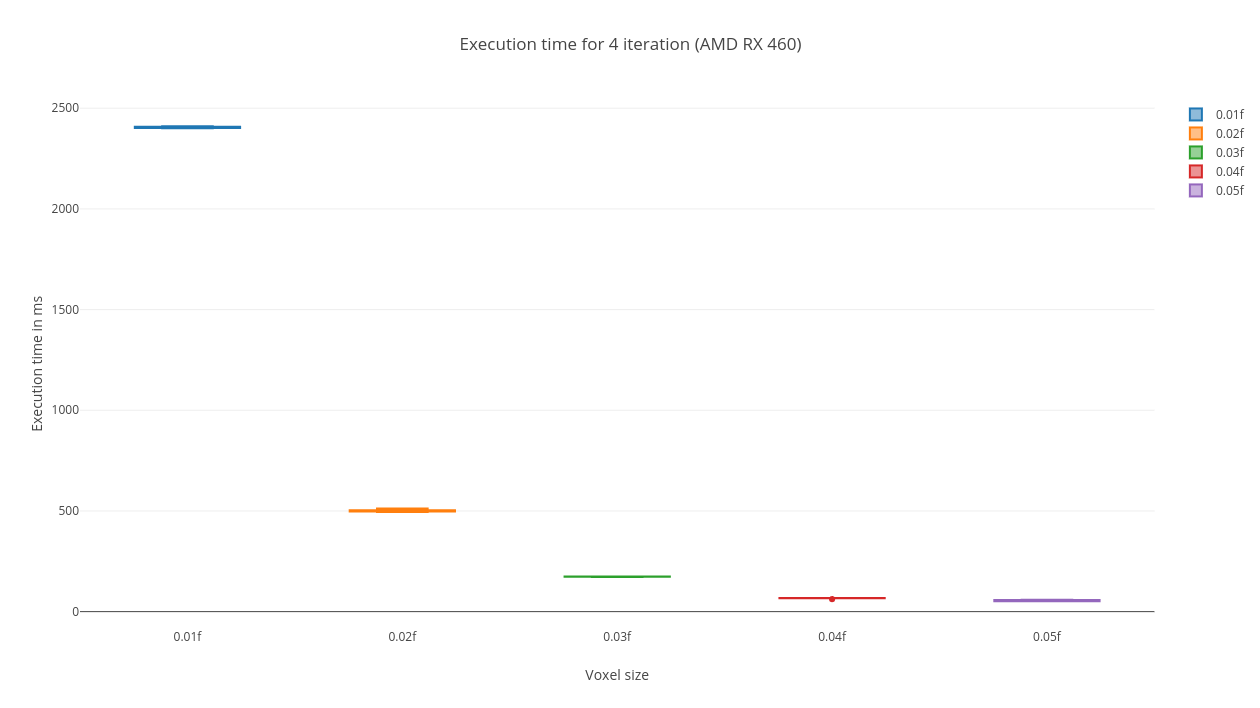
\includegraphics[width=14cm]{images/AllfouriterationRX460.png}
	\caption{Execution time for 4 iterations with AMD RX460}
	\label{ExampleOCTImage}
\end{figure}
\pagebreak
And with the second setup, NVIDIA TITAN X:

\begin{figure}[H]
	\centering
	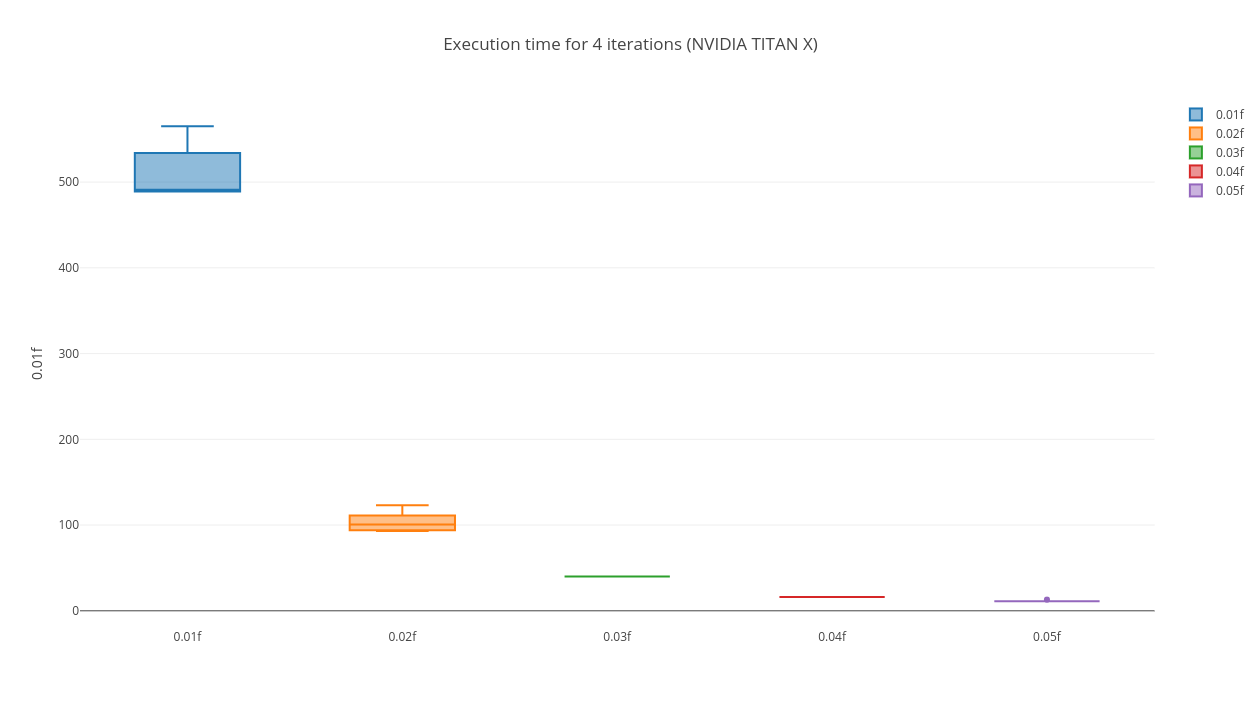
\includegraphics[width=14cm]{images/AllfourIterationTITANX.png}
	\caption{Execution time for 4 iterations with NVIDIA TITAN X}
	\label{ExampleOCTImage}
\end{figure}

In the two illustrations the vertical axis stands for the execution time for all iterations in milliseconds and the horizontal axis stands for resolution of the point clouds. The size of points in source and model point clouds directly depend on the solution, with concrete numbers presented as following :



\begin{table}[H]
\centering
\caption{Point cloud sizes with corresponding resolution}
\label{my-label}
\begin{tabular}{llllll}
Resolution         & 0.01f & 0.02f & 0.03f & 0.04f & 0.05f \\
Source Point cloud & 9037  & 2289  & 1159  & 557   & 462   \\
Model Point Cloud  & 2037  & 1225  & 716   & 428   & 283  
\end{tabular}
\end{table}
\newpage
The results show a notable correlation between the resolution and execution time :  The bigger the size of model and source point clouds, the slower the execution. A dramatic change could be seen between 0.02f and 0.01f, when the size of source point cloud quadruples its size and the model has almost two times more points. These difference in model size heavily changes the time needed to reserve memory and execute kernels. However, a closer investigation in execution time in these steps shows a different changes between them : bigger sized model and source point cloud slow down the second step (finding correspondence) drastically, whereas does not have much effect on to first (transforming point cloud) and third step (sum up result). The difference lies between the tasks of those kernels : While first and third step are independent from the point cloud sizes, the second step is about looping through the source point cloud to find correspondence, which consequently would take longer for bigger point cloud. 

For the resolution used in the example, which is 0.02f, the performance of each step mentioned in the last chapter, is presented in the following figures, start with the AMD setup:

\begin{figure}[H]
	\centering
	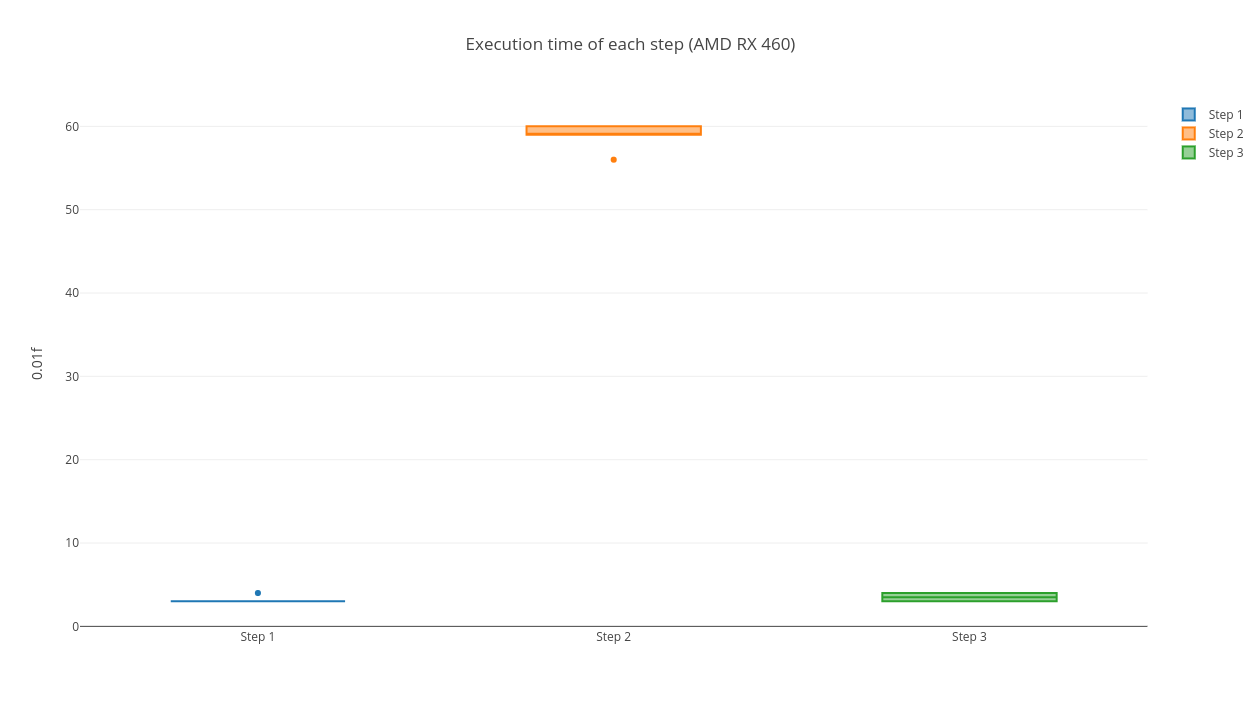
\includegraphics[width=14cm]{images/EachstepAMD.png}
	\caption{Execution time for each step with AMD RX460}
	\label{ExampleOCTImage}
\end{figure}
\newpage
And for NVIDIA setup:

\begin{figure}[H]
	\centering
	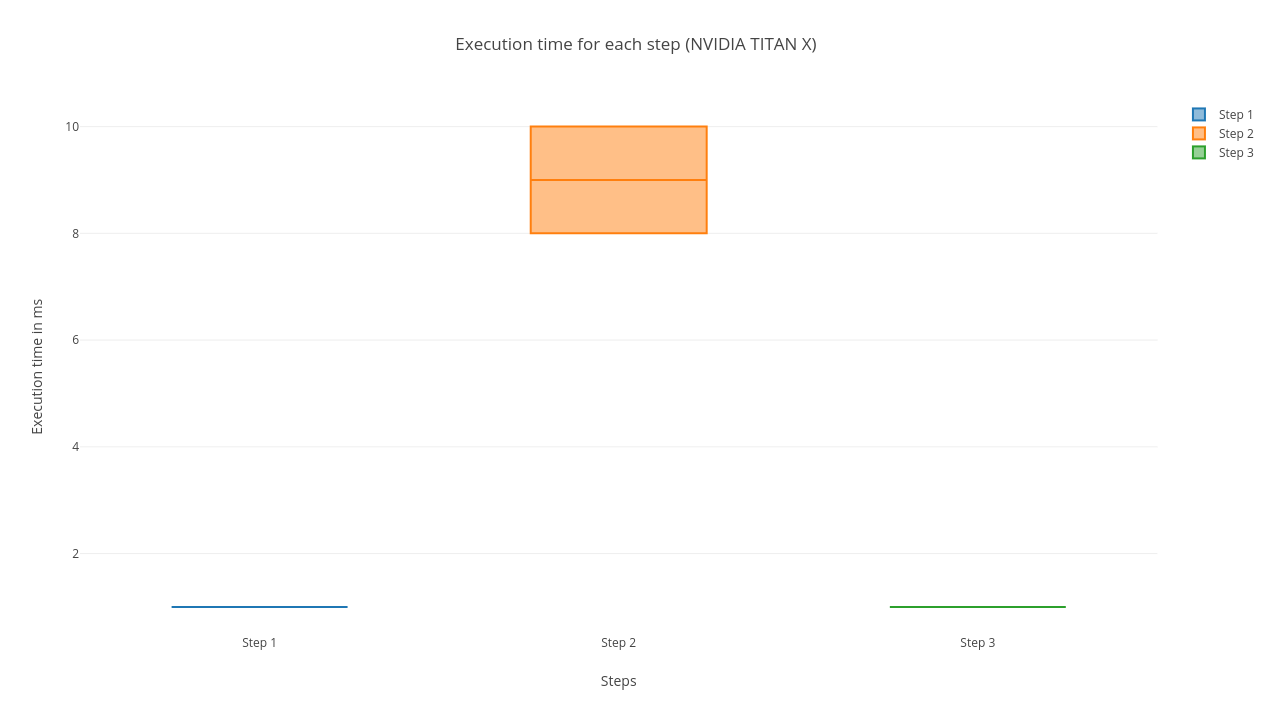
\includegraphics[width=14cm]{images/EachStepNVIDIA.png}
	\caption{Execution time for each step with NVIDIA TITANX}
	\label{ExampleOCTImage}
\end{figure}

A significant improvement in performance in step 2 shows how computational resource demanding the kernel function is. It often takes up to 90\% of total performance time and shows the best improvements with better hardware. The execution time in this step depends solely and heavily on the clock speed of each processing unit and access speed to the global memory of the physical device.

In conclusion, the OpenCL Implementation shows a better performance than the CPU implementation. It is roughly 15-20x times faster for the NVIDIA setup and 4-5x times faster for a AMD setup, with both of these devices available for off the shelf purchase. It also opens up the possibility of using more than GPU devices and reduce the workload of the CPU. The end performance is far more reliable and is a step forward in development of the robotic system. 

The possibility of a better result does not stop there, since the GPU still has not used all available computing power. A potentially better strategy to parallelize the task by using more work units might result into a much better execution time, or a different approach can be applied in the second step, the most time consuming part of the algorithm. However, within the scope of this thesis, another approach will not be investigated and leaves room for improvement in further development. 



\input{components/sources}


\bibliographystyle{plain}
\bibliography{References}
\end{document}